\documentclass[../calc1-main.tex]{subfiles}

\begin{document}

  Suppose you drive in 2 hours from city A to city B which are 200km apart. That means your average speed was 100km/h. Even if you did not travel constant speed, there was at least one instant where  your speed was exactly 100km/h. This is called \textbf{mean value theorem}.

  \begin{minipage}{0.5\textwidth}
    \begin{theorem}[The Mean-Value Theorem]
      Suppose that $f$ is continuous on the interval $[a, b]$ and that it is differentiable on the open interval $(a, b)$. Then there exists a point $c$ in the open interval $(a, b)$ s.t.
      \[
        \frac{f(b) - f(a)}{b - a} = f'(c).
      \]
    \end{theorem}
  \end{minipage}%
  \begin{minipage}{0.5\textwidth}
    \begin{figure}[H]
      \centering
      \tikzset{point/.style={circle,draw=black,inner sep=0pt,minimum size=3pt}}

\begin{tikzpicture}
    \draw[thick] (1,1) node[point,fill=black] (a) {} parabola bend (3,3) (4,2.5) node[point,fill=black] (b) {};
    \draw[thick] (1,1) -- (4,2.5);
    \draw (1,1+9/8) -- (4,2.5+9/8) coordinate (topright);
    \node[point,fill=black] (c) at (2.5,2.875) {};

    \coordinate (origin) at (0,0);
    \draw[<->] (topright -| origin) -- (origin) -- (origin -| topright) -- +(1,0);
    \draw[dotted,very thick] (a) -- (a|-origin) node[below,black] {$a$};
    \draw[dotted,very thick] (b) -- (b|-origin) node[below] {$b$};
    \draw[dashed] (c) -- (c|-origin) node[below] {$c$};
\end{tikzpicture}
      \caption{Mean Value Theorem says that the slope of the secant line joining two points on the graph of of $f(x)$ is equal to the slope of the tangent line at some point $x=c$ between $a$ and $b$.}
    \end{figure}
  \end{minipage}

  Let $f(t)$ denote the distance from city A. Then $f(0) = 0$ and $f(2) = 200$. Mean Value Theorem says there is a time $t = c$ s.t. $f'(c) = 100$.

  \begin{example}
    Let $f(x) = \abs{x}$ on $[-1, 1]$. Show that there is no $c \in [-1, 1]$ satisfying the conclusion of the Mean Value Theorem. Why?
  \end{example}

  The Mean Value Theorem is an \textit{existence theorem} like Intermediate Value Theorem. In particular
  \begin{itemize}
    \item We don't know how to find $c$.
    \item We don't know how many different $c$ can be found satisfying Mean Value Theorem (there is at least one).
    \begin{figure}[H]
      \centering
      \tikzset{point/.style={circle,draw=black,inner sep=0pt,minimum size=3pt}}
\begin{tikzpicture}
    \begin{scope}
    \clip (-3,-2) rectangle (3,2);
    \draw[thick,smooth,domain=-3:3] plot (\x,{\x^3/3 - \x});
    \end{scope}
    \node[point,fill=black] (a) at (-2,-2/3) {};
    \node[point,fill=black] (b) at (2,2/3) {};
    \draw[thick] (a) -- (b);
    \coordinate (origin) at (-4,-3);
    \coordinate (topright) at (4,2);
    \draw[<->] (topright -| origin) -- (origin) -- (origin -| topright);
    \draw[dotted,very thick] (a) -- (a|-origin) node[below] {$a$};
    \draw[dotted,very thick] (b) -- (b|-origin) node[below] {$b$};

    \node[point,fill=black] (c0) at ({-2/sqrt(3)},{(1/3)*(-2/sqrt(3))^3+2/sqrt(3)}) {};
    \draw (c0) +(-1,-1/3) -- +(1,1/3);
    \node[point,fill=black] (c1) at ({2/sqrt(3)},{(1/3)*(2/sqrt(3))^3-2/sqrt(3)}) {};
    \draw (c1) +(-1,-1/3) -- +(1,1/3);
    \draw[dashed] (c0) -- (c0 |- origin) node[below]{$c_0$};
    \draw[dashed] (c1) -- (c1 |- origin) node[below]{$c_1$};
\end{tikzpicture}
      \caption{There may be more than one $c$ satisfying the conclusion of the Mean Value Theorem.}
    \end{figure}
  \end{itemize}

  \begin{example}
    Show that $\sin x < x$ for all $x>0$.
  \end{example}
  \begin{solution}
    For $x > 2\pi$, we have $\sin x < 1 < 2\pi < x$. Now assume $0<x<2\pi$. By the Mean Value Theorem there exists $c$, $0<c<x$ such that
    \[
      \frac{\sin x - \sin 0}{x-0} = \cos c.
    \]
    Hence $\sin x = x \cos c$. Since $0<c<2\pi$, $\cos c < 1$. Since also $x >0$, we have $x \cos c < x$. So $\sin x = x \cos c < x$.
  \end{solution}

  \begin{example}
    Show that $\sqrt{1+x} < 1 + \frac{x}{2}$ for all $x>0$.
  \end{example}
  \begin{solution}
    Let $f(x) = \sqrt{1+x}$. Then $f'(c) < \frac{1}{2}$ for $c>0$. Use Mean Value Theorem.
  \end{solution}

  \begin{example}
    Determine all the numbers $c$ which satisfy the conclusions of the Mean Value Theorem for
    \[
      f(x) = x^3 + 2x^2 -x, \qquad x\in[-1,2]
    \]
  \end{example}
  \begin{solution}
    Solve
    \[
      3c^2 + 4c - 1 = f'(c) = \frac{f(2)-f(-1)}{2-(-1)} = \frac{14-2}{3} = 4
    \]
    Solutions of $3c^2+4c-5=0$ are
    \[
      c_{\pm} = \frac{-4 \pm \sqrt{76}}{6}.
    \]
    Notice that only $\frac{-4 + \sqrt{76}}{6}$ lies in $[-1,2]$.
  \end{solution}
  \begin{example}
    Suppose $f$ is continuous and differentiable on $[3, 9]$. Suppose $f(3)=-4$, and $f'(x) \le 10$ for all $x$. What is the largest value possible for $f(9)$?
  \end{example}
  \begin{solution}
    By Mean Value Theorem, there exists $c \in (3,9)$ such that
    \[
      f(9)-f(3) = f'(c) (9-3) \le 10 \times 6 = 60.
    \]
    So $f(9) \le 60 + f(3) = 56$.
  \end{solution}

  \begin{definition}
    Suppose $f$ is defined on an interval $I$. If for all $x_1, x_2$ in $I$ s.t. $x_2 > x_1$,
    \begin{table}[H]
      \centering
      \begin{tabular}{|c|c|}
        \hline
        If & Then on $I$, $f$ is \\
        \hline
        $f(x_2) > f(x_1)$ & increasing \\
        $f(x_2) < f(x_1)$ & decreasing \\
        $f(x_2) \ge f(x_1)$ & non-decreasing \\
        $f(x_2) \le f(x_1)$ & non-increasing \\
        \hline
      \end{tabular}
    \end{table}
  \end{definition}

  \begin{theorem}
    Suppose $f$ is differentiable on an open interval $I$. If for all $x \in I$,
    \begin{table}[H]
      \centering
      \begin{tabular}{|c|c|}
        \hline
        If & Then on $I$, $f$ is \\
        \hline
        $f'(x) > 0$ & increasing \\
        $f'(x) < 0$ & decreasing \\
        $f'(x) \ge 0$ & non-decreasing \\
        $f'(x) \le 0$ & non-increasing \\
        \hline
      \end{tabular}
    \end{table}

  \end{theorem}
  \begin{proof}
    Let's prove the first statement. Let $x_2 > x_1$ in $I$. By the Mean Value Theorem, there exists $c$, $x_1< c < x_2$, such that $f(x_2) - f(x_1) = f'(c) (x_2 - x_1)$. Since $f'(c)>0$  and $x_2-x_1>0$, we have $f(x_2) > f_(x_1)$. So $f$ is increasing.
  \end{proof}

  \begin{example}
    On what intervals is $f(x) = x^3 - 12 x + 1$ increasing or decreasing?
  \end{example}
  \begin{solution}
    ~\\
    \begin{minipage}{0.5\textwidth}
      $f'(x) = 3(x-2)(x+2)$. So $f$ is decreasing on $(-2, 2)$ and increasing otherwise.
    \end{minipage}%
    \begin{minipage}{0.5\textwidth}
      \begin{figure}[H]
        \centering
        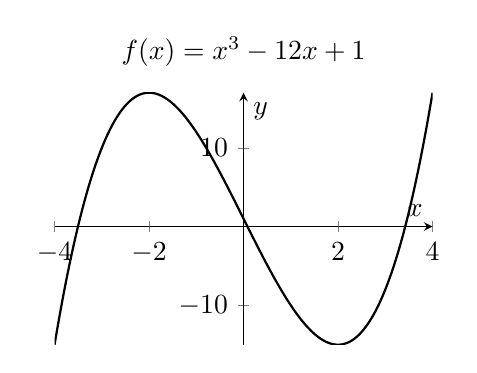
\begin{tikzpicture}
  \begin{axis}[
  axis lines=middle, % left, right, box, center, none
  x=6mm,
  y=1mm,
  title={$f(x)=x^3-12x+1$},
  xlabel=$x$,
  ylabel=$y$
  ]
  \addplot[domain=-4:4, thick, samples=250] {x^3-12*x+1};
\end{axis}
\end{tikzpicture}
      \end{figure}
    \end{minipage}

  \end{solution}

  We know that if $f$ is a constant function then its derivative is zero. The converse is also true.
  \begin{theorem} \label{THM: functions with zero derivative are constant}
    If $f'(x) = 0$ on an interval $I$ then $f(x)$ is constant on $I$.
  \end{theorem}
  \begin{proof}
    Choose $x_0$ in $I$. Let $C = f(x_0)$. If $x$ is any other point in $I$ then by Mean Value Theorem, $f(x) - f(x_0) = f'(c) (x-x_0) = 0$.
  \end{proof}
\end{document}
